\documentclass[10pt]{article}

\usepackage{caption}
\usepackage{subcaption}
\usepackage{graphicx}

\begin{document}

\section{Exercise 1}

Gradient descent is an iterative procedure to find the local minimum of a function $f(x)$ by successively looking at values of the function proportional to the direction of the gradient of the function. The iteration stops when the result from two successive steps yields a difference below a specified threshold. This means that once the local minimum is reached, movement along the gradient of a given function will not yield significantly different results. For a scalar function with vector argument inputs, this procedure can be written mathematically as: 
$$x_{n + 1} = x_n - \eta*\nabla f(x_n).$$

A start value $x_0$ and a step size $\eta$ is given to start the procedure, as well as a threshold $\beta$. When $|x_{n + 1} - x_n| < \beta$, the procedure stops. It is possible to define different step sizes $\eta$ for each iteration of the gradient descent procedure, but this analysis assumes a constant step size. 

Testing this gradient descent optimizer on an upside-down Gaussian function with mean $6$ and variance $4$, we expect the minimum to occur at $(6, -1)$, since there is one global minimum. If the function and gradient are defined as: 
$$f(x) = -e^{\frac{(x - 6)^2}{8}} \qquad \nabla f = \frac{x - 6}{4} e^{\frac{(x - 6)^2}{8}}$$
(see Figure \ref{fig:gaus}), then the gradient descent algorithm always converges to the correct global minimum. For functions with one minimum, the larger the step value, the faster the algorithm will converge, regardless of how far the initial guess is from the minimum. The threshold dictates how close the numerical solution is from the analytical solution (see Figure \ref{tbl:gaus}).

\begin{figure}[!ht]
	\centering
	\makebox[\linewidth][c]{%}
	\begin{subfigure}[h]{0.55\textwidth}
	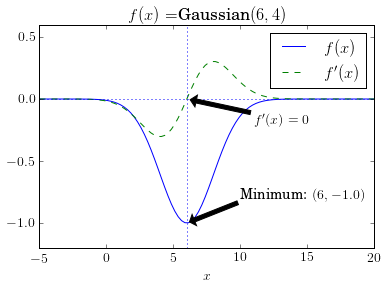
\includegraphics[width=\textwidth]{exercise1a.png}
	\caption{Graph of $f(x)$ and its gradient}
	\label{fig:gaus}
	\end{subfigure}
	\begin{subtable}[h]{0.55\textwidth}
	\centering
	\vspace{12mm}
	\begin{tabular}[h]{cccc}
		Guess & Step & Iterations & Minimum \\\hline
		5 & 0.5 & 21 & (5.934, -.999) \\\hline
		5 & 1 & 13 & (5.974, -1.000)  \\\hline
		2 & 0.5 & 47 & (5.938, -1.000) \\\hline
		2 & 5 & 4 & (5.998, -1.000) \\\hline
	\end{tabular}
	\vspace{12mm}
	\caption{Parameters and results of gradient descent. The threshold was always $0.01$}
	\label{tbl:gaus}
	\end{subtable}
	}\\
	\caption{Results for $f(x) = $-Gaussian$(6, 4)$}
\end{figure}

The same algorithm can be applied to scalar functions with vector inputs. For example, 
$$ f(x, y) = (x + 2)^2 + y^2 \qquad \nabla f = 2(x + 2) + 2y$$
And has one global minimum. In choosing parameters, the smaller the step size and the smaller the threshold, the more iterations are required for the algorithm to converge.

\begin{figure}[!ht]
	\centering
	\makebox[\linewidth][c]{%}min}
	\begin{subfigure}[b]{0.55\textwidth}
		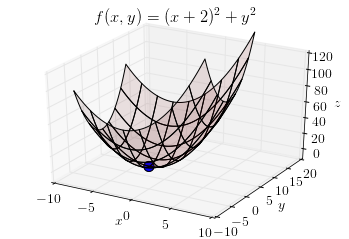
\includegraphics[width=\textwidth]{exercise1c.png}
		\caption{$f(x, y)$, $\nabla f$, and the estimated minimum}
		\label{fig:nomin}
	\end{subfigure}
	\begin{subtable}[b]{0.55\textwidth}
	\centering
	\begin{tabular}[b]{ccccc}
		Guess & Step & Thresh & Iterations \\\hline
		(0, 0) & 0.5 & 0.01 & 2 \\\hline
		(5, 5) & 0.5 & 0.01 & 2  \\\hline
		(5, 5) & 0.1 & 0.01 & 25 \\\hline
		(5, 5) & 0.1 & 0.001 & 35 \\\hline
	\end{tabular}
	\vspace{10mm}
	\caption{Parameters and results of gradient descent. The minimum always came out to be $(-2, 0, 0)$}
	\label{tbl:nomin}
	\end{subtable}
	}\\
	\caption{Using gradient descent to estimate the minimum of a scalar function with vector inputs}
\end{figure}

For functions without a global minimum (non-convex functions), the choice of input parameters dictates not only how fast the algorithm converges, but also the value at which it converges. For example, the function
$$f(x) = \sin(x + \frac{\pi}{2}) + 3 \qquad \nabla f = \cos(x + \frac{\pi}{2})$$
has local minima at $(2(n + 1)\pi, 2)$ for all $n$ (see Figure \ref{fig:nomin}). When the initial guess for gradient descent is chosen to be closer to the local minima at $-\pi$, the algorithm estimates that to be the local minimum, and vice versa for $\pi$. If the initial guess is given at $0$, which is a local maximum, the algorithm does not descend and stops after one iteration.

\begin{figure}[!ht]
	\centering
	\makebox[\linewidth][c]{%}min}
	\begin{subfigure}[b]{0.6\textwidth}
		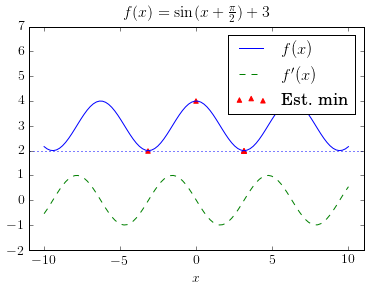
\includegraphics[width=\textwidth]{exercise1d.png}
		\caption{$f(x)$, $\nabla f$, and the estimated minima}
		\label{fig:2var}
	\end{subfigure}
	\begin{subtable}[b]{0.6\textwidth}
	\centering
	\begin{tabular}[b]{ccccc}
		Guess & Step & Thresh & Iterations & Minimum \\\hline
		5 & 0.5 & 0.01 & 9 & ($\pi$, 2) \\\hline
		-5 & 0.5 & 0.01 & 9 & ($-\pi$, 2)  \\\hline
		0 & 0.5 & 0.01 & 1 & (0, 4) \\\hline
		0.5 & 0.5 & 0.01 & 12 & ($\pi$, 2) \\\hline
		0.2 & 0.5 & 0.01 & 14 & ($\pi$, 2) \\\hline
		0.7 & 0.5 & 0.01 & 11 & ($\pi$, 2) \\\hline
	\end{tabular}
	\vspace{10mm}
	\caption{Parameters and results of gradient descent}
	\label{tbl:nomin}
	\end{subtable}
	}\\
	\caption{Using gradient descent on a function with many local minima}
\end{figure}

\begin{figure}[!ht]
\centering
	\makebox[\linewidth][c]{%}min}
\begin{subfigure}[ht]{0.4\textwidth}
		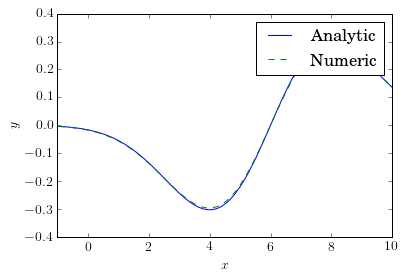
\includegraphics[width=\textwidth]{exercise1e.png}
		\label{fig:cdgaus}
		\caption{}
	\end{subfigure}
	\begin{subfigure}[ht]{0.4\textwidth}
		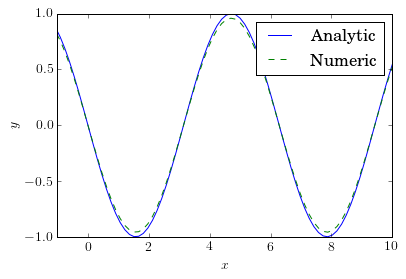
\includegraphics[width=\textwidth]{exercise1f.png}
		\label{fig:cdsin}
		\caption{}
	\end{subfigure}
	\begin{subtable}[ht]{0.4\textwidth}
	\centering
	\begin{tabular}[ht]{ccccc}
		(x, y) & Analytic $\nabla f$ & Numeric\\\hline
		(-2, -2) & (0, -4) & (0, -4) \\\hline
		(-2, -1) & (0, -2) & (0, -2) \\\hline
		(-2, 0) & (0, 0) & (0, 0) \\\hline
		(-2, 1) & (0, 2) & (0, 2) \\\hline
		(-2, 2) & (0, 4) & (0, 4) \\\hline
	\end{tabular}
	\vspace{5mm}
	\label{tbl:2varcd}
	\caption{}
	\end{subtable}
	}\\
	\label{fig:centraldiff}
	\caption{The step size for calculating the central difference was $1$. (a) The analytic and numeric approximations of Figure \ref{fig:gaus}. (b) The analytic and numeric approximations of Figure \ref{fig:nomin}.  (c) The analytic and numeric approximations of Figure \ref{fig:2var}.}
\end{figure}

The gradient of a function can either be specified analytically or numerically approximated with central differences using $\delta_{h}[f](x) = f(x + 0.5h) - f(x - 0.5h)$. From a numerical standpoint, using either the analytical or numerical approximation to the gradient is approximately equivalent, given the correct choice of step size (see Figure 4).

\begin{table}[!ht]
\centering
\begin{tabular}[ht]{cccc}
Function & Algorithm & Guess & Iterations \\\hline
$f(x) = -$Gaussian$(6, 4)$ & GD & 5 & 21 \\
$f(x) = -$Gaussian$(6, 4)$ & \textsc{BFGS} & 5 & 6 \\
$f(x) = \sin(x + \frac{\pi}{2}) + 3$ & GD & 5 & 9 \\
$f(x) = \sin(x + \frac{\pi}{2}) + 3$ & \textsc{BFGS} & 5 & 4 \\
$f(x, y) = (x + 2)^2 + y^2$ & GD & (5, 5) & 25 \\
$f(x, y) = (x + 2)^2 + y^2$ & \textsc{BFGS} & (5, 5) & 2 \\
\end{tabular}
\label{tbl:bfgs}
\caption{Steps to convergence. GD is gradient descent, \textsc{BFGS} is from SciPy.}
\end{table}

Software packages like SciPy implement a different algorithm for estimating minima. Table 1 gives a comparison of the number of iterations of the algorithm needed to find a solution. In general, the \textsc{bfgs} optimizer in SciPy performs better than the simple gradient descent algorithm presented here. Both algorithms came up to the same solution within a few significant digits.

\newpage
\section{Exercise 2}

This is a test. 

\section{Exercise 3}

This is a test. 

\section{Exercise 4}

This is a test. 

\end{document}